\documentclass{report}

%%%%%%%%%%%%%%%%%%%%%%%%%%%%%%%%%
% PACKAGE IMPORTS
%%%%%%%%%%%%%%%%%%%%%%%%%%%%%%%%%


\usepackage[tmargin=2cm,rmargin=1in,lmargin=1in,margin=0.85in,bmargin=2cm,footskip=.2in]{geometry}
\usepackage{amsmath,amsfonts,amsthm,amssymb,mathtools}
\usepackage[varbb]{newpxmath}
\usepackage{xfrac}
\usepackage[makeroom]{cancel}
\usepackage{mathtools}
\usepackage{bookmark}
\usepackage{enumitem}
\usepackage{hyperref,theoremref}
\hypersetup{
	pdftitle={Assignment},
	colorlinks=true, linkcolor=violet,
	bookmarksnumbered=true,
	bookmarksopen=true
}
\usepackage[most,many,breakable]{tcolorbox}
\usepackage{xcolor}
\usepackage{varwidth}
\usepackage{varwidth}
\usepackage{etoolbox}
%\usepackage{authblk}
\usepackage{nameref}
\usepackage{multicol,array}
\usepackage{tikz-cd}
\usepackage[ruled,vlined,linesnumbered]{algorithm2e}
\usepackage{comment} % enables the use of multi-line comments (\ifx \fi) 
\usepackage{import}
\usepackage{xifthen}
\usepackage{pdfpages}
\usepackage{transparent}
\usepackage{afterpage}

\newcommand\mycommfont[1]{\footnotesize\ttfamily\textcolor{violet}{#1}}
\SetCommentSty{mycommfont}
\newcommand{\incfig}[1]{%
    \def\svgwidth{\columnwidth}
    \import{./figures/}{#1.pdf_tex}
}

\usepackage{tikzsymbols}
\renewcommand\qedsymbol{$\Laughey$}


%\usepackage{import}
%\usepackage{xifthen}
%\usepackage{pdfpages}
%\usepackage{transparent}

%%%%%%%%%%%%%%%%%%%%%%%%%%%%%%
% TEX LIVE PACKAGES
%%%%%%%%%%%%%%%%%%%%%%%%%%%%%%

\usepackage[T1]{fontenc}
\usepackage{anyfontsize}

%%%%%%%%%%%%%%%%%%%%%%%%%%%%%%
% BLANK PAGE
%%%%%%%%%%%%%%%%%%%%%%%%%%%%%%

\newcommand\blankpage{%
    \null
    \thispagestyle{empty}%
    \addtocounter{page}{-1}%
    \newpage
}

%%%%%%%%%%%%%%%%%%%%%%%%%%%%%%
% SELF MADE COLORS
%%%%%%%%%%%%%%%%%%%%%%%%%%%%%%



\definecolor{myg}{RGB}{56, 140, 70}
\definecolor{myb}{RGB}{45, 111, 177}
\definecolor{myr}{RGB}{199, 68, 64}
\definecolor{mytheorembg}{HTML}{F2F2F9}
\definecolor{mytheoremfr}{HTML}{00007B}
\definecolor{mylenmabg}{HTML}{FFFAF8}
\definecolor{mylenmafr}{HTML}{983b0f}
\definecolor{mypropbg}{HTML}{f2fbfc}
\definecolor{mypropfr}{HTML}{191971}
\definecolor{myexamplebg}{HTML}{F2FBF8}
\definecolor{myexamplefr}{HTML}{88D6D1}
\definecolor{myexampleti}{HTML}{2A7F7F}
\definecolor{mydefinitbg}{HTML}{E5E5FF}
\definecolor{mydefinitfr}{HTML}{3F3FA3}
\definecolor{notesred}{RGB}{0,162,0}
\definecolor{myp}{RGB}{197, 92, 212}
\definecolor{mygr}{HTML}{2C3338}
\definecolor{myred}{RGB}{127,0,0}
\definecolor{myyellow}{RGB}{169,121,69}
\definecolor{myexercisebg}{HTML}{F2FBF8}
\definecolor{myexercisefg}{HTML}{88D6D1}


%%%%%%%%%%%%%%%%%%%%%%%%%%%%
% TCOLORBOX SETUPS
%%%%%%%%%%%%%%%%%%%%%%%%%%%%

\setlength{\parindent}{1cm}
%================================
% THEOREM BOX
%================================

\tcbuselibrary{theorems,skins,hooks}
\newtcbtheorem[number within=section]{Theorem}{Teorema}
{%
	enhanced,
	breakable,
	colback = mytheorembg,
	frame hidden,
	boxrule = 0sp,
	borderline west = {2pt}{0pt}{mytheoremfr},
	sharp corners,
	detach title,
	before upper = \tcbtitle\par\smallskip,
	coltitle = mytheoremfr,
	fonttitle = \bfseries\sffamily,
	description font = \mdseries,
	separator sign none,
	segmentation style={solid, mytheoremfr},
}
{th}

\tcbuselibrary{theorems,skins,hooks}
\newtcbtheorem[number within=chapter]{theorem}{Theorem}
{%
	enhanced,
	breakable,
	colback = mytheorembg,
	frame hidden,
	boxrule = 0sp,
	borderline west = {2pt}{0pt}{mytheoremfr},
	sharp corners,
	detach title,
	before upper = \tcbtitle\par\smallskip,
	coltitle = mytheoremfr,
	fonttitle = \bfseries\sffamily,
	description font = \mdseries,
	separator sign none,
	segmentation style={solid, mytheoremfr},
}
{th}


\tcbuselibrary{theorems,skins,hooks}
\newtcolorbox{Theoremcon}
{%
	enhanced
	,breakable
	,colback = mytheorembg
	,frame hidden
	,boxrule = 0sp
	,borderline west = {2pt}{0pt}{mytheoremfr}
	,sharp corners
	,description font = \mdseries
	,separator sign none
}

%================================
% Corollery
%================================
\tcbuselibrary{theorems,skins,hooks}
\newtcbtheorem[number within=section]{Corollary}{Corollario}
{%
	enhanced
	,breakable
	,colback = myp!10
	,frame hidden
	,boxrule = 0sp
	,borderline west = {2pt}{0pt}{myp!85!black}
	,sharp corners
	,detach title
	,before upper = \tcbtitle\par\smallskip
	,coltitle = myp!85!black
	,fonttitle = \bfseries\sffamily
	,description font = \mdseries
	,separator sign none
	,segmentation style={solid, myp!85!black}
}
{th}
\tcbuselibrary{theorems,skins,hooks}
\newtcbtheorem[number within=chapter]{corollary}{Corollary}
{%
	enhanced
	,breakable
	,colback = myp!10
	,frame hidden
	,boxrule = 0sp
	,borderline west = {2pt}{0pt}{myp!85!black}
	,sharp corners
	,detach title
	,before upper = \tcbtitle\par\smallskip
	,coltitle = myp!85!black
	,fonttitle = \bfseries\sffamily
	,description font = \mdseries
	,separator sign none
	,segmentation style={solid, myp!85!black}
}
{th}


%================================
% LENMA
%================================

\tcbuselibrary{theorems,skins,hooks}
\newtcbtheorem[number within=section]{Lenma}{Lenma}
{%
	enhanced,
	breakable,
	colback = mylenmabg,
	frame hidden,
	boxrule = 0sp,
	borderline west = {2pt}{0pt}{mylenmafr},
	sharp corners,
	detach title,
	before upper = \tcbtitle\par\smallskip,
	coltitle = mylenmafr,
	fonttitle = \bfseries\sffamily,
	description font = \mdseries,
	separator sign none,
	segmentation style={solid, mylenmafr},
}
{th}

\tcbuselibrary{theorems,skins,hooks}
\newtcbtheorem[number within=chapter]{lenma}{Lenma}
{%
	enhanced,
	breakable,
	colback = mylenmabg,
	frame hidden,
	boxrule = 0sp,
	borderline west = {2pt}{0pt}{mylenmafr},
	sharp corners,
	detach title,
	before upper = \tcbtitle\par\smallskip,
	coltitle = mylenmafr,
	fonttitle = \bfseries\sffamily,
	description font = \mdseries,
	separator sign none,
	segmentation style={solid, mylenmafr},
}
{th}


%================================
% PROPOSITION
%================================

\tcbuselibrary{theorems,skins,hooks}
\newtcbtheorem[number within=section]{Prop}{Proposition}
{%
	enhanced,
	breakable,
	colback = mypropbg,
	frame hidden,
	boxrule = 0sp,
	borderline west = {2pt}{0pt}{mypropfr},
	sharp corners,
	detach title,
	before upper = \tcbtitle\par\smallskip,
	coltitle = mypropfr,
	fonttitle = \bfseries\sffamily,
	description font = \mdseries,
	separator sign none,
	segmentation style={solid, mypropfr},
}
{th}

\tcbuselibrary{theorems,skins,hooks}
\newtcbtheorem[number within=chapter]{prop}{Proposition}
{%
	enhanced,
	breakable,
	colback = mypropbg,
	frame hidden,
	boxrule = 0sp,
	borderline west = {2pt}{0pt}{mypropfr},
	sharp corners,
	detach title,
	before upper = \tcbtitle\par\smallskip,
	coltitle = mypropfr,
	fonttitle = \bfseries\sffamily,
	description font = \mdseries,
	separator sign none,
	segmentation style={solid, mypropfr},
}
{th}


%================================
% CLAIM
%================================

\tcbuselibrary{theorems,skins,hooks}
\newtcbtheorem[number within=section]{claim}{Claim}
{%
	enhanced
	,breakable
	,colback = myg!10
	,frame hidden
	,boxrule = 0sp
	,borderline west = {2pt}{0pt}{myg}
	,sharp corners
	,detach title
	,before upper = \tcbtitle\par\smallskip
	,coltitle = myg!85!black
	,fonttitle = \bfseries\sffamily
	,description font = \mdseries
	,separator sign none
	,segmentation style={solid, myg!85!black}
}
{th}



%================================
% Exercise
%================================

\tcbuselibrary{theorems,skins,hooks}
\newtcbtheorem[number within=section]{Exercise}{Exercise}
{%
	enhanced,
	breakable,
	colback = myexercisebg,
	frame hidden,
	boxrule = 0sp,
	borderline west = {2pt}{0pt}{myexercisefg},
	sharp corners,
	detach title,
	before upper = \tcbtitle\par\smallskip,
	coltitle = myexercisefg,
	fonttitle = \bfseries\sffamily,
	description font = \mdseries,
	separator sign none,
	segmentation style={solid, myexercisefg},
}
{th}

\tcbuselibrary{theorems,skins,hooks}
\newtcbtheorem[number within=chapter]{exercise}{Exercise}
{%
	enhanced,
	breakable,
	colback = myexercisebg,
	frame hidden,
	boxrule = 0sp,
	borderline west = {2pt}{0pt}{myexercisefg},
	sharp corners,
	detach title,
	before upper = \tcbtitle\par\smallskip,
	coltitle = myexercisefg,
	fonttitle = \bfseries\sffamily,
	description font = \mdseries,
	separator sign none,
	segmentation style={solid, myexercisefg},
}
{th}

%================================
% EXAMPLE BOX
%================================

\newtcbtheorem[number within=section]{Example}{Esempio}
{%
	colback = myexamplebg
	,breakable
	,colframe = myexamplefr
	,coltitle = myexampleti
	,boxrule = 1pt
	,sharp corners
	,detach title
	,before upper=\tcbtitle\par\smallskip
	,fonttitle = \bfseries
	,description font = \mdseries
	,separator sign none
	,description delimiters parenthesis
}
{ex}

\newtcbtheorem[number within=chapter]{example}{Esempio}
{%
	colback = myexamplebg
	,breakable
	,colframe = myexamplefr
	,coltitle = myexampleti
	,boxrule = 1pt
	,sharp corners
	,detach title
	,before upper=\tcbtitle\par\smallskip
	,fonttitle = \bfseries
	,description font = \mdseries
	,separator sign none
	,description delimiters parenthesis
}
{ex}

%================================
% DEFINITION BOX
%================================

\newtcbtheorem[number within=section]{Definizione}{Definizione}{enhanced,
	before skip=2mm,after skip=2mm, colback=red!5,colframe=red!80!black,boxrule=0.5mm,
	attach boxed title to top left={xshift=1cm,yshift*=1mm-\tcboxedtitleheight}, varwidth boxed title*=-3cm,
	boxed title style={frame code={
					\path[fill=tcbcolback]
					([yshift=-1mm,xshift=-1mm]frame.north west)
					arc[start angle=0,end angle=180,radius=1mm]
					([yshift=-1mm,xshift=1mm]frame.north east)
					arc[start angle=180,end angle=0,radius=1mm];
					\path[left color=tcbcolback!60!black,right color=tcbcolback!60!black,
						middle color=tcbcolback!80!black]
					([xshift=-2mm]frame.north west) -- ([xshift=2mm]frame.north east)
					[rounded corners=1mm]-- ([xshift=1mm,yshift=-1mm]frame.north east)
					-- (frame.south east) -- (frame.south west)
					-- ([xshift=-1mm,yshift=-1mm]frame.north west)
					[sharp corners]-- cycle;
				},interior engine=empty,
		},
	fonttitle=\bfseries,
	title={#2},#1}{def}
\newtcbtheorem[number within=chapter]{definizione}{Definizione}{enhanced,
	before skip=2mm,after skip=2mm, colback=red!5,colframe=red!80!black,boxrule=0.5mm,
	attach boxed title to top left={xshift=1cm,yshift*=1mm-\tcboxedtitleheight}, varwidth boxed title*=-3cm,
	boxed title style={frame code={
					\path[fill=tcbcolback]
					([yshift=-1mm,xshift=-1mm]frame.north west)
					arc[start angle=0,end angle=180,radius=1mm]
					([yshift=-1mm,xshift=1mm]frame.north east)
					arc[start angle=180,end angle=0,radius=1mm];
					\path[left color=tcbcolback!60!black,right color=tcbcolback!60!black,
						middle color=tcbcolback!80!black]
					([xshift=-2mm]frame.north west) -- ([xshift=2mm]frame.north east)
					[rounded corners=1mm]-- ([xshift=1mm,yshift=-1mm]frame.north east)
					-- (frame.south east) -- (frame.south west)
					-- ([xshift=-1mm,yshift=-1mm]frame.north west)
					[sharp corners]-- cycle;
				},interior engine=empty,
		},
	fonttitle=\bfseries,
	title={#2},#1}{def}



%================================
% Solution BOX
%================================

\makeatletter
\newtcbtheorem{question}{Question}{enhanced,
	breakable,
	colback=white,
	colframe=myb!80!black,
	attach boxed title to top left={yshift*=-\tcboxedtitleheight},
	fonttitle=\bfseries,
	title={#2},
	boxed title size=title,
	boxed title style={%
			sharp corners,
			rounded corners=northwest,
			colback=tcbcolframe,
			boxrule=0pt,
		},
	underlay boxed title={%
			\path[fill=tcbcolframe] (title.south west)--(title.south east)
			to[out=0, in=180] ([xshift=5mm]title.east)--
			(title.center-|frame.east)
			[rounded corners=\kvtcb@arc] |-
			(frame.north) -| cycle;
		},
	#1
}{def}
\makeatother

%================================
% SOLUTION BOX
%================================

\makeatletter
\newtcolorbox{solution}{enhanced,
	breakable,
	colback=white,
	colframe=myg!80!black,
	attach boxed title to top left={yshift*=-\tcboxedtitleheight},
	title=Solution,
	boxed title size=title,
	boxed title style={%
			sharp corners,
			rounded corners=northwest,
			colback=tcbcolframe,
			boxrule=0pt,
		},
	underlay boxed title={%
			\path[fill=tcbcolframe] (title.south west)--(title.south east)
			to[out=0, in=180] ([xshift=5mm]title.east)--
			(title.center-|frame.east)
			[rounded corners=\kvtcb@arc] |-
			(frame.north) -| cycle;
		},
}
\makeatother

%================================
% Question BOX
%================================

\makeatletter
\newtcbtheorem{qstion}{Question}{enhanced,
	breakable,
	colback=white,
	colframe=mygr,
	attach boxed title to top left={yshift*=-\tcboxedtitleheight},
	fonttitle=\bfseries,
	title={#2},
	boxed title size=title,
	boxed title style={%
			sharp corners,
			rounded corners=northwest,
			colback=tcbcolframe,
			boxrule=0pt,
		},
	underlay boxed title={%
			\path[fill=tcbcolframe] (title.south west)--(title.south east)
			to[out=0, in=180] ([xshift=5mm]title.east)--
			(title.center-|frame.east)
			[rounded corners=\kvtcb@arc] |-
			(frame.north) -| cycle;
		},
	#1
}{def}
\makeatother

\newtcbtheorem[number within=chapter]{wconc}{Wrong Concept}{
	breakable,
	enhanced,
	colback=white,
	colframe=myr,
	arc=0pt,
	outer arc=0pt,
	fonttitle=\bfseries\sffamily\large,
	colbacktitle=myr,
	attach boxed title to top left={},
	boxed title style={
			enhanced,
			skin=enhancedfirst jigsaw,
			arc=3pt,
			bottom=0pt,
			interior style={fill=myr}
		},
	#1
}{def}



%================================
% NOTE BOX
%================================

\usetikzlibrary{arrows,calc,shadows.blur}
\tcbuselibrary{skins}
\newtcolorbox{note}[1][]{%
	enhanced jigsaw,
	colback=gray!20!white,%
	colframe=gray!80!black,
	size=small,
	boxrule=1pt,
	title=\textbf{Note:-},
	halign title=flush center,
	coltitle=black,
	breakable,
	drop shadow=black!50!white,
	attach boxed title to top left={xshift=1cm,yshift=-\tcboxedtitleheight/2,yshifttext=-\tcboxedtitleheight/2},
	minipage boxed title=1.5cm,
	boxed title style={%
			colback=white,
			size=fbox,
			boxrule=1pt,
			boxsep=2pt,
			underlay={%
					\coordinate (dotA) at ($(interior.west) + (-0.5pt,0)$);
					\coordinate (dotB) at ($(interior.east) + (0.5pt,0)$);
					\begin{scope}
						\clip (interior.north west) rectangle ([xshift=3ex]interior.east);
						\filldraw [white, blur shadow={shadow opacity=60, shadow yshift=-.75ex}, rounded corners=2pt] (interior.north west) rectangle (interior.south east);
					\end{scope}
					\begin{scope}[gray!80!black]
						\fill (dotA) circle (2pt);
						\fill (dotB) circle (2pt);
					\end{scope}
				},
		},
	#1,
}

%%%%%%%%%%%%%%%%%%%%%%%%%%%%%%
% SELF MADE COMMANDS
%%%%%%%%%%%%%%%%%%%%%%%%%%%%%%


\newcommand{\thm}[2]{\begin{Theorem}{#1}{}#2\end{Theorem}}
\newcommand{\cor}[2]{\begin{Corollary}{#1}{}#2\end{Corollary}}
\newcommand{\mlenma}[2]{\begin{Lenma}{#1}{}#2\end{Lenma}}
\newcommand{\mprop}[2]{\begin{Prop}{#1}{}#2\end{Prop}}
\newcommand{\clm}[3]{\begin{claim}{#1}{#2}#3\end{claim}}
\newcommand{\wc}[2]{\begin{wconc}{#1}{}\setlength{\parindent}{1cm}#2\end{wconc}}
\newcommand{\thmcon}[1]{\begin{Theoremcon}{#1}\end{Theoremcon}}
\newcommand{\ex}[2]{\begin{Example}{#1}{}#2\end{Example}}
\newcommand{\dfn}[2]{\begin{Definizione}[colbacktitle=red!75!black]{#1}{}#2\end{Definizione}}
\newcommand{\dfnc}[2]{\begin{definizione}[colbacktitle=red!75!black]{#1}{}#2\end{definizione}}
\newcommand{\qs}[2]{\begin{question}{#1}{}#2\end{question}}
\newcommand{\pf}[2]{\begin{myproof}[#1]#2\end{myproof}}
\newcommand{\nt}[1]{\begin{note}#1\end{note}}

\newcommand*\circled[1]{\tikz[baseline=(char.base)]{
		\node[shape=circle,draw,inner sep=1pt] (char) {#1};}}
\newcommand\getcurrentref[1]{%
	\ifnumequal{\value{#1}}{0}
	{??}
	{\the\value{#1}}%
}
\newcommand{\getCurrentSectionNumber}{\getcurrentref{section}}
\newenvironment{myproof}[1][\proofname]{%
	\proof[\bfseries #1: ]%
}{\endproof}

\newcommand{\mclm}[2]{\begin{myclaim}[#1]#2\end{myclaim}}
\newenvironment{myclaim}[1][\claimname]{\proof[\bfseries #1: ]}{}

\newcounter{mylabelcounter}

\makeatletter
\newcommand{\setword}[2]{%
	\phantomsection
	#1\def\@currentlabel{\unexpanded{#1}}\label{#2}%
}
\makeatother




\tikzset{
	symbol/.style={
			draw=none,
			every to/.append style={
					edge node={node [sloped, allow upside down, auto=false]{$#1$}}}
		}
}


% deliminators
\DeclarePairedDelimiter{\abs}{\lvert}{\rvert}
\DeclarePairedDelimiter{\norm}{\lVert}{\rVert}

\DeclarePairedDelimiter{\ceil}{\lceil}{\rceil}
\DeclarePairedDelimiter{\floor}{\lfloor}{\rfloor}
\DeclarePairedDelimiter{\round}{\lfloor}{\rceil}

\newsavebox\diffdbox
\newcommand{\slantedromand}{{\mathpalette\makesl{d}}}
\newcommand{\makesl}[2]{%
\begingroup
\sbox{\diffdbox}{$\mathsurround=0pt#1\mathrm{#2}$}%
\pdfsave
\pdfsetmatrix{1 0 0.2 1}%
\rlap{\usebox{\diffdbox}}%
\pdfrestore
\hskip\wd\diffdbox
\endgroup
}
\newcommand{\dd}[1][]{\ensuremath{\mathop{}\!\ifstrempty{#1}{%
\slantedromand\@ifnextchar^{\hspace{0.2ex}}{\hspace{0.1ex}}}%
{\slantedromand\hspace{0.2ex}^{#1}}}}
\ProvideDocumentCommand\dv{o m g}{%
  \ensuremath{%
    \IfValueTF{#3}{%
      \IfNoValueTF{#1}{%
        \frac{\dd #2}{\dd #3}%
      }{%
        \frac{\dd^{#1} #2}{\dd #3^{#1}}%
      }%
    }{%
      \IfNoValueTF{#1}{%
        \frac{\dd}{\dd #2}%
      }{%
        \frac{\dd^{#1}}{\dd #2^{#1}}%
      }%
    }%
  }%
}
\providecommand*{\pdv}[3][]{\frac{\partial^{#1}#2}{\partial#3^{#1}}}
%  - others
\DeclareMathOperator{\Lap}{\mathcal{L}}
\DeclareMathOperator{\Var}{Var} % varience
\DeclareMathOperator{\Cov}{Cov} % covarience
\DeclareMathOperator{\E}{E} % expected

% Since the amsthm package isn't loaded

% I prefer the slanted \leq
\let\oldleq\leq % save them in case they're every wanted
\let\oldgeq\geq
\renewcommand{\leq}{\leqslant}
\renewcommand{\geq}{\geqslant}

% % redefine matrix env to allow for alignment, use r as default
% \renewcommand*\env@matrix[1][r]{\hskip -\arraycolsep
%     \let\@ifnextchar\new@ifnextchar
%     \array{*\c@MaxMatrixCols #1}}


%\usepackage{framed}
%\usepackage{titletoc}
%\usepackage{etoolbox}
%\usepackage{lmodern}


%\patchcmd{\tableofcontents}{\contentsname}{\sffamily\contentsname}{}{}

%\renewenvironment{leftbar}
%{\def\FrameCommand{\hspace{6em}%
%		{\color{myyellow}\vrule width 2pt depth 6pt}\hspace{1em}}%
%	\MakeFramed{\parshape 1 0cm \dimexpr\textwidth-6em\relax\FrameRestore}\vskip2pt%
%}
%{\endMakeFramed}

%\titlecontents{chapter}
%[0em]{\vspace*{2\baselineskip}}
%{\parbox{4.5em}{%
%		\hfill\Huge\sffamily\bfseries\color{myred}\thecontentspage}%
%	\vspace*{-2.3\baselineskip}\leftbar\textsc{\small\chaptername~\thecontentslabel}\\\sffamily}
%{}{\endleftbar}
%\titlecontents{section}
%[8.4em]
%{\sffamily\contentslabel{3em}}{}{}
%{\hspace{0.5em}\nobreak\itshape\color{myred}\contentspage}
%\titlecontents{subsection}
%[8.4em]
%{\sffamily\contentslabel{3em}}{}{}  
%{\hspace{0.5em}\nobreak\itshape\color{myred}\contentspage}



%%%%%%%%%%%%%%%%%%%%%%%%%%%%%%%%%%%%%%%%%%%
% TABLE OF CONTENTS
%%%%%%%%%%%%%%%%%%%%%%%%%%%%%%%%%%%%%%%%%%%

\usepackage{tikz}
\definecolor{doc}{RGB}{0,60,110}
\usepackage{titletoc}
\contentsmargin{0cm}
\titlecontents{chapter}[3.7pc]
{\addvspace{30pt}%
	\begin{tikzpicture}[remember picture, overlay]%
		\draw[fill=violet,draw=violet] (-7.3,-.1) rectangle (-0.5,.5);%
		\pgftext[left,x=-3.7cm,y=0.2cm]{\color{white}\Large\sc\bfseries Capitolo\ \thecontentslabel};%
	\end{tikzpicture}\color{violet}\large\sc\bfseries}%
{}
{}
{\;\titlerule\;\large\sc\bfseries Pagina \thecontentspage
	\begin{tikzpicture}[remember picture, overlay]
		\draw[fill=violet,draw=violet] (2pt,0) rectangle (4,0.1pt);
	\end{tikzpicture}}%
\titlecontents{section}[3.7pc]
{\addvspace{2pt}}
{\contentslabel[\thecontentslabel]{2pc}}
{}
{\hfill\small \thecontentspage}
[]
\titlecontents*{subsection}[3.7pc]
{\addvspace{-1pt}\small}
{}
{}
{\ --- \small\thecontentspage}
[ \textbullet\ ][]

\makeatletter
\renewcommand{\chaptername}{Capitolo}
\renewcommand{\tableofcontents}{%
	\chapter*{%
	  \vspace*{-20\p@}%
	  \begin{tikzpicture}[remember picture, overlay]%
		  \pgftext[right,x=15cm,y=0.2cm]{\color{violet}\Huge\sc\bfseries \contentsname};%
		  \draw[fill=violet,draw=violet] (13,-.75) rectangle (20,1);%
		  \clip (13,-.75) rectangle (20,1);
		  \pgftext[right,x=15cm,y=0.2cm]{\color{white}\Huge\sc\bfseries \contentsname};%
	  \end{tikzpicture}}%
	\@starttoc{toc}}
\makeatother

%%%%%%%%%%%%%%%%%%%%%%%%%%%%%%%%%%%%%%%%%%%
% HYPERLINK
%%%%%%%%%%%%%%%%%%%%%%%%%%%%%%%%%%%%%%%%%%%

\hypersetup{
    colorlinks,
    citecolor=black,
    filecolor=black,
    linkcolor=black,
    urlcolor=black
}
%From M275 "Topology" at SJSU
\newcommand{\id}{\mathrm{id}}
\newcommand{\taking}[1]{\xrightarrow{#1}}
\newcommand{\inv}{^{-1}}

%From M170 "Introduction to Graph Theory" at SJSU
\DeclareMathOperator{\diam}{diam}
\DeclareMathOperator{\ord}{ord}
\newcommand{\defeq}{\overset{\mathrm{def}}{=}}

%From the USAMO .tex files
\newcommand{\ts}{\textsuperscript}
\newcommand{\dg}{^\circ}
\newcommand{\ii}{\item}

% % From Math 55 and Math 145 at Harvard
% \newenvironment{subproof}[1][Proof]{%
% \begin{proof}[#1] \renewcommand{\qedsymbol}{$\blacksquare$}}%
% {\end{proof}}

\newcommand{\ac}{\Leftrightarrow_\alpha}
\newcommand{\br}{\rightarrow_\beta}
\newcommand{\er}{\rightarrow_\eta}
\newcommand{\liff}{\leftrightarrow}
\newcommand{\lthen}{\rightarrow}
\newcommand{\opname}{\operatorname}
\newcommand{\surjto}{\twoheadrightarrow}
\newcommand{\injto}{\hookrightarrow}
\newcommand{\On}{\mathrm{On}} % ordinals
\DeclareMathOperator{\img}{im} % Image
\DeclareMathOperator{\Img}{Im} % Image
\DeclareMathOperator{\coker}{coker} % Cokernel
\DeclareMathOperator{\Coker}{Coker} % Cokernel
\DeclareMathOperator{\Ker}{Ker} % Kernel
\DeclareMathOperator{\rank}{rank}
\DeclareMathOperator{\Spec}{Spec} % spectrum
\DeclareMathOperator{\Tr}{Tr} % trace
\DeclareMathOperator{\pr}{pr} % projection
\DeclareMathOperator{\ext}{ext} % extension
\DeclareMathOperator{\pred}{pred} % predecessor
\DeclareMathOperator{\dom}{dom} % domain
\DeclareMathOperator{\ran}{ran} % range
\DeclareMathOperator{\Hom}{Hom} % homomorphism
\DeclareMathOperator{\Mor}{Mor} % morphisms
\DeclareMathOperator{\End}{End} % endomorphism

\newcommand{\eps}{\epsilon}
\newcommand{\veps}{\varepsilon}
\newcommand{\ol}{\overline}
\newcommand{\ul}{\underline}
\newcommand{\wt}{\widetilde}
\newcommand{\wh}{\widehat}
\newcommand{\vocab}[1]{\textbf{\color{blue} #1}}
\providecommand{\half}{\frac{1}{2}}
\newcommand{\dang}{\measuredangle} %% Directed angle
\newcommand{\ray}[1]{\overrightarrow{#1}}
\newcommand{\seg}[1]{\overline{#1}}
\newcommand{\arc}[1]{\wideparen{#1}}
\DeclareMathOperator{\cis}{cis}
\DeclareMathOperator*{\lcm}{lcm}
\DeclareMathOperator*{\argmin}{arg min}
\DeclareMathOperator*{\argmax}{arg max}
\newcommand{\cycsum}{\sum_{\mathrm{cyc}}}
\newcommand{\symsum}{\sum_{\mathrm{sym}}}
\newcommand{\cycprod}{\prod_{\mathrm{cyc}}}
\newcommand{\symprod}{\prod_{\mathrm{sym}}}
\newcommand{\Qed}{\begin{flushright}\qed\end{flushright}}
\newcommand{\parinn}{\setlength{\parindent}{1cm}}
\newcommand{\parinf}{\setlength{\parindent}{0cm}}
% \newcommand{\norm}{\|\cdot\|}
\newcommand{\inorm}{\norm_{\infty}}
\newcommand{\opensets}{\{V_{\alpha}\}_{\alpha\in I}}
\newcommand{\oset}{V_{\alpha}}
\newcommand{\opset}[1]{V_{\alpha_{#1}}}
\newcommand{\lub}{\text{lub}}
\newcommand{\del}[2]{\frac{\partial #1}{\partial #2}}
\newcommand{\Del}[3]{\frac{\partial^{#1} #2}{\partial^{#1} #3}}
\newcommand{\deld}[2]{\dfrac{\partial #1}{\partial #2}}
\newcommand{\Deld}[3]{\dfrac{\partial^{#1} #2}{\partial^{#1} #3}}
\newcommand{\lm}{\lambda}
\newcommand{\uin}{\mathbin{\rotatebox[origin=c]{90}{$\in$}}}
\newcommand{\usubset}{\mathbin{\rotatebox[origin=c]{90}{$\subset$}}}
\newcommand{\lt}{\left}
\newcommand{\rt}{\right}
\newcommand{\bs}[1]{\boldsymbol{#1}}
\newcommand{\exs}{\exists}
\newcommand{\st}{\strut}
\newcommand{\dps}[1]{\displaystyle{#1}}

\newcommand{\sol}{\setlength{\parindent}{0cm}\textbf{\textit{Solution:}}\setlength{\parindent}{1cm} }
\newcommand{\solve}[1]{\setlength{\parindent}{0cm}\textbf{\textit{Solution: }}\setlength{\parindent}{1cm}#1 \Qed}
% Things Lie
\newcommand{\kb}{\mathfrak b}
\newcommand{\kg}{\mathfrak g}
\newcommand{\kh}{\mathfrak h}
\newcommand{\kn}{\mathfrak n}
\newcommand{\ku}{\mathfrak u}
\newcommand{\kz}{\mathfrak z}
\DeclareMathOperator{\Ext}{Ext} % Ext functor
\DeclareMathOperator{\Tor}{Tor} % Tor functor
\newcommand{\gl}{\opname{\mathfrak{gl}}} % frak gl group
\renewcommand{\sl}{\opname{\mathfrak{sl}}} % frak sl group chktex 6

% More script letters etc.
\newcommand{\SA}{\mathcal A}
\newcommand{\SB}{\mathcal B}
\newcommand{\SC}{\mathcal C}
\newcommand{\SF}{\mathcal F}
\newcommand{\SG}{\mathcal G}
\newcommand{\SH}{\mathcal H}
\newcommand{\OO}{\mathcal O}

\newcommand{\SCA}{\mathscr A}
\newcommand{\SCB}{\mathscr B}
\newcommand{\SCC}{\mathscr C}
\newcommand{\SCD}{\mathscr D}
\newcommand{\SCE}{\mathscr E}
\newcommand{\SCF}{\mathscr F}
\newcommand{\SCG}{\mathscr G}
\newcommand{\SCH}{\mathscr H}

% Mathfrak primes
\newcommand{\km}{\mathfrak m}
\newcommand{\kp}{\mathfrak p}
\newcommand{\kq}{\mathfrak q}

% number sets
\newcommand{\RR}[1][]{\ensuremath{\ifstrempty{#1}{\mathbb{R}}{\mathbb{R}^{#1}}}}
\newcommand{\NN}[1][]{\ensuremath{\ifstrempty{#1}{\mathbb{N}}{\mathbb{N}^{#1}}}}
\newcommand{\ZZ}[1][]{\ensuremath{\ifstrempty{#1}{\mathbb{Z}}{\mathbb{Z}^{#1}}}}
\newcommand{\QQ}[1][]{\ensuremath{\ifstrempty{#1}{\mathbb{Q}}{\mathbb{Q}^{#1}}}}
\newcommand{\CC}[1][]{\ensuremath{\ifstrempty{#1}{\mathbb{C}}{\mathbb{C}^{#1}}}}
\newcommand{\PP}[1][]{\ensuremath{\ifstrempty{#1}{\mathbb{P}}{\mathbb{P}^{#1}}}}
\newcommand{\HH}[1][]{\ensuremath{\ifstrempty{#1}{\mathbb{H}}{\mathbb{H}^{#1}}}}
\newcommand{\FF}[1][]{\ensuremath{\ifstrempty{#1}{\mathbb{F}}{\mathbb{F}^{#1}}}}
% expected value
\newcommand{\EE}{\ensuremath{\mathbb{E}}}
\newcommand{\charin}{\text{ char }}
\DeclareMathOperator{\sign}{sign}
\DeclareMathOperator{\Aut}{Aut}
\DeclareMathOperator{\Inn}{Inn}
\DeclareMathOperator{\Syl}{Syl}
\DeclareMathOperator{\Gal}{Gal}
\DeclareMathOperator{\GL}{GL} % General linear group
\DeclareMathOperator{\SL}{SL} % Special linear group

%---------------------------------------
% BlackBoard Math Fonts :-
%---------------------------------------

%Captital Letters
\newcommand{\bbA}{\mathbb{A}}	\newcommand{\bbB}{\mathbb{B}}
\newcommand{\bbC}{\mathbb{C}}	\newcommand{\bbD}{\mathbb{D}}
\newcommand{\bbE}{\mathbb{E}}	\newcommand{\bbF}{\mathbb{F}}
\newcommand{\bbG}{\mathbb{G}}	\newcommand{\bbH}{\mathbb{H}}
\newcommand{\bbI}{\mathbb{I}}	\newcommand{\bbJ}{\mathbb{J}}
\newcommand{\bbK}{\mathbb{K}}	\newcommand{\bbL}{\mathbb{L}}
\newcommand{\bbM}{\mathbb{M}}	\newcommand{\bbN}{\mathbb{N}}
\newcommand{\bbO}{\mathbb{O}}	\newcommand{\bbP}{\mathbb{P}}
\newcommand{\bbQ}{\mathbb{Q}}	\newcommand{\bbR}{\mathbb{R}}
\newcommand{\bbS}{\mathbb{S}}	\newcommand{\bbT}{\mathbb{T}}
\newcommand{\bbU}{\mathbb{U}}	\newcommand{\bbV}{\mathbb{V}}
\newcommand{\bbW}{\mathbb{W}}	\newcommand{\bbX}{\mathbb{X}}
\newcommand{\bbY}{\mathbb{Y}}	\newcommand{\bbZ}{\mathbb{Z}}

%---------------------------------------
% MathCal Fonts :-
%---------------------------------------

%Captital Letters
\newcommand{\mcA}{\mathcal{A}}	\newcommand{\mcB}{\mathcal{B}}
\newcommand{\mcC}{\mathcal{C}}	\newcommand{\mcD}{\mathcal{D}}
\newcommand{\mcE}{\mathcal{E}}	\newcommand{\mcF}{\mathcal{F}}
\newcommand{\mcG}{\mathcal{G}}	\newcommand{\mcH}{\mathcal{H}}
\newcommand{\mcI}{\mathcal{I}}	\newcommand{\mcJ}{\mathcal{J}}
\newcommand{\mcK}{\mathcal{K}}	\newcommand{\mcL}{\mathcal{L}}
\newcommand{\mcM}{\mathcal{M}}	\newcommand{\mcN}{\mathcal{N}}
\newcommand{\mcO}{\mathcal{O}}	\newcommand{\mcP}{\mathcal{P}}
\newcommand{\mcQ}{\mathcal{Q}}	\newcommand{\mcR}{\mathcal{R}}
\newcommand{\mcS}{\mathcal{S}}	\newcommand{\mcT}{\mathcal{T}}
\newcommand{\mcU}{\mathcal{U}}	\newcommand{\mcV}{\mathcal{V}}
\newcommand{\mcW}{\mathcal{W}}	\newcommand{\mcX}{\mathcal{X}}
\newcommand{\mcY}{\mathcal{Y}}	\newcommand{\mcZ}{\mathcal{Z}}


%---------------------------------------
% Bold Math Fonts :-
%---------------------------------------

%Captital Letters
\newcommand{\bmA}{\boldsymbol{A}}	\newcommand{\bmB}{\boldsymbol{B}}
\newcommand{\bmC}{\boldsymbol{C}}	\newcommand{\bmD}{\boldsymbol{D}}
\newcommand{\bmE}{\boldsymbol{E}}	\newcommand{\bmF}{\boldsymbol{F}}
\newcommand{\bmG}{\boldsymbol{G}}	\newcommand{\bmH}{\boldsymbol{H}}
\newcommand{\bmI}{\boldsymbol{I}}	\newcommand{\bmJ}{\boldsymbol{J}}
\newcommand{\bmK}{\boldsymbol{K}}	\newcommand{\bmL}{\boldsymbol{L}}
\newcommand{\bmM}{\boldsymbol{M}}	\newcommand{\bmN}{\boldsymbol{N}}
\newcommand{\bmO}{\boldsymbol{O}}	\newcommand{\bmP}{\boldsymbol{P}}
\newcommand{\bmQ}{\boldsymbol{Q}}	\newcommand{\bmR}{\boldsymbol{R}}
\newcommand{\bmS}{\boldsymbol{S}}	\newcommand{\bmT}{\boldsymbol{T}}
\newcommand{\bmU}{\boldsymbol{U}}	\newcommand{\bmV}{\boldsymbol{V}}
\newcommand{\bmW}{\boldsymbol{W}}	\newcommand{\bmX}{\boldsymbol{X}}
\newcommand{\bmY}{\boldsymbol{Y}}	\newcommand{\bmZ}{\boldsymbol{Z}}
%Small Letters
\newcommand{\bma}{\boldsymbol{a}}	\newcommand{\bmb}{\boldsymbol{b}}
\newcommand{\bmc}{\boldsymbol{c}}	\newcommand{\bmd}{\boldsymbol{d}}
\newcommand{\bme}{\boldsymbol{e}}	\newcommand{\bmf}{\boldsymbol{f}}
\newcommand{\bmg}{\boldsymbol{g}}	\newcommand{\bmh}{\boldsymbol{h}}
\newcommand{\bmi}{\boldsymbol{i}}	\newcommand{\bmj}{\boldsymbol{j}}
\newcommand{\bmk}{\boldsymbol{k}}	\newcommand{\bml}{\boldsymbol{l}}
\newcommand{\bmm}{\boldsymbol{m}}	\newcommand{\bmn}{\boldsymbol{n}}
\newcommand{\bmo}{\boldsymbol{o}}	\newcommand{\bmp}{\boldsymbol{p}}
\newcommand{\bmq}{\boldsymbol{q}}	\newcommand{\bmr}{\boldsymbol{r}}
\newcommand{\bms}{\boldsymbol{s}}	\newcommand{\bmt}{\boldsymbol{t}}
\newcommand{\bmu}{\boldsymbol{u}}	\newcommand{\bmv}{\boldsymbol{v}}
\newcommand{\bmw}{\boldsymbol{w}}	\newcommand{\bmx}{\boldsymbol{x}}
\newcommand{\bmy}{\boldsymbol{y}}	\newcommand{\bmz}{\boldsymbol{z}}

%---------------------------------------
% Scr Math Fonts :-
%---------------------------------------

\newcommand{\sA}{{\mathscr{A}}}   \newcommand{\sB}{{\mathscr{B}}}
\newcommand{\sC}{{\mathscr{C}}}   \newcommand{\sD}{{\mathscr{D}}}
\newcommand{\sE}{{\mathscr{E}}}   \newcommand{\sF}{{\mathscr{F}}}
\newcommand{\sG}{{\mathscr{G}}}   \newcommand{\sH}{{\mathscr{H}}}
\newcommand{\sI}{{\mathscr{I}}}   \newcommand{\sJ}{{\mathscr{J}}}
\newcommand{\sK}{{\mathscr{K}}}   \newcommand{\sL}{{\mathscr{L}}}
\newcommand{\sM}{{\mathscr{M}}}   \newcommand{\sN}{{\mathscr{N}}}
\newcommand{\sO}{{\mathscr{O}}}   \newcommand{\sP}{{\mathscr{P}}}
\newcommand{\sQ}{{\mathscr{Q}}}   \newcommand{\sR}{{\mathscr{R}}}
\newcommand{\sS}{{\mathscr{S}}}   \newcommand{\sT}{{\mathscr{T}}}
\newcommand{\sU}{{\mathscr{U}}}   \newcommand{\sV}{{\mathscr{V}}}
\newcommand{\sW}{{\mathscr{W}}}   \newcommand{\sX}{{\mathscr{X}}}
\newcommand{\sY}{{\mathscr{Y}}}   \newcommand{\sZ}{{\mathscr{Z}}}


%---------------------------------------
% Math Fraktur Font
%---------------------------------------

%Captital Letters
\newcommand{\mfA}{\mathfrak{A}}	\newcommand{\mfB}{\mathfrak{B}}
\newcommand{\mfC}{\mathfrak{C}}	\newcommand{\mfD}{\mathfrak{D}}
\newcommand{\mfE}{\mathfrak{E}}	\newcommand{\mfF}{\mathfrak{F}}
\newcommand{\mfG}{\mathfrak{G}}	\newcommand{\mfH}{\mathfrak{H}}
\newcommand{\mfI}{\mathfrak{I}}	\newcommand{\mfJ}{\mathfrak{J}}
\newcommand{\mfK}{\mathfrak{K}}	\newcommand{\mfL}{\mathfrak{L}}
\newcommand{\mfM}{\mathfrak{M}}	\newcommand{\mfN}{\mathfrak{N}}
\newcommand{\mfO}{\mathfrak{O}}	\newcommand{\mfP}{\mathfrak{P}}
\newcommand{\mfQ}{\mathfrak{Q}}	\newcommand{\mfR}{\mathfrak{R}}
\newcommand{\mfS}{\mathfrak{S}}	\newcommand{\mfT}{\mathfrak{T}}
\newcommand{\mfU}{\mathfrak{U}}	\newcommand{\mfV}{\mathfrak{V}}
\newcommand{\mfW}{\mathfrak{W}}	\newcommand{\mfX}{\mathfrak{X}}
\newcommand{\mfY}{\mathfrak{Y}}	\newcommand{\mfZ}{\mathfrak{Z}}
%Small Letters
\newcommand{\mfa}{\mathfrak{a}}	\newcommand{\mfb}{\mathfrak{b}}
\newcommand{\mfc}{\mathfrak{c}}	\newcommand{\mfd}{\mathfrak{d}}
\newcommand{\mfe}{\mathfrak{e}}	\newcommand{\mff}{\mathfrak{f}}
\newcommand{\mfg}{\mathfrak{g}}	\newcommand{\mfh}{\mathfrak{h}}
\newcommand{\mfi}{\mathfrak{i}}	\newcommand{\mfj}{\mathfrak{j}}
\newcommand{\mfk}{\mathfrak{k}}	\newcommand{\mfl}{\mathfrak{l}}
\newcommand{\mfm}{\mathfrak{m}}	\newcommand{\mfn}{\mathfrak{n}}
\newcommand{\mfo}{\mathfrak{o}}	\newcommand{\mfp}{\mathfrak{p}}
\newcommand{\mfq}{\mathfrak{q}}	\newcommand{\mfr}{\mathfrak{r}}
\newcommand{\mfs}{\mathfrak{s}}	\newcommand{\mft}{\mathfrak{t}}
\newcommand{\mfu}{\mathfrak{u}}	\newcommand{\mfv}{\mathfrak{v}}
\newcommand{\mfw}{\mathfrak{w}}	\newcommand{\mfx}{\mathfrak{x}}
\newcommand{\mfy}{\mathfrak{y}}	\newcommand{\mfz}{\mathfrak{z}}

\renewcommand{\contentsname}{Indice}

\title{\Huge{Programmazione III}}
\author{\huge{Luca Barra}}
\date{Anno accademico 2023/2024}

\begin{document}

\maketitle
\newpage% or \cleardoublepage
% \pdfbookmark[<level>]{<title>}{<dest>}
\pdfbookmark[section]{\contentsname}{toc}
\afterpage{\blankpage}
\pagenumbering{Roman}
\tableofcontents
\cleardoublepage\pagenumbering{arabic}
\pagebreak
\afterpage{\blankpage}

\chapter{Introduzione}

\section{Tipi di paradigmi di programmazione}

\begin{center}
    \begin{tabular}{ | l | p{7cm} | p{5cm} |}
    \hline
    \textbf{Paradigma}      
& \textbf{Un programma è}
& \textbf{Esempi} \\ \hline\hline
Imperativo
& Sequenza di azioni (esecuzione $\Rightarrow$ nuovo stato)
& C, C++, Pascal, Java, Scala, Python, Scheme\\ \hline
Object-oriented
& Oggetti che comunicano (interazione $\Rightarrow$ nuovo stato)
& Smalltalk, C++, OCaml, Java, Scala, Python \\ \hline
Funzionale
& Espressione (valutazione $\Rightarrow$ risultato)
& Haskell, OCaml, Scala, Erlang, Scheme \\
    \hline
    \end{tabular}
\end{center}

\noindent Per il paradigma \textit{imperativo} un programma è una sequenza di azioni che modificano lo stato attuale del calcolatore. Per il paradigma \textit{object-oriented} un programma è un insieme di oggetti che comunicano tra loro tramite uno scambio di messaggi. Per il paradigma \textit{funzionale} un programma è una grande espressione in cui compaiono funzioni. Un programma funzionale si \textit{valuta}, non si esegue.
Quasi tutti i linguaggi attuali sono \textit{multi-paradigma}, ossia hanno caratteristiche di due o più paradigmi.

\section{I linguaggi funzionali}

\subsection{Il \texorpdfstring{$\mathcal{\lambda}$}--calcolo}

La programmazione \textit{funzionale} risale agli anni '30, prima della costruzione dei primi calcolatori elettronici. Il \textit{$\lambda$-calcolo}\footnote{Il "$\lambda$" nasce da un errore tipografico, doveva essere un accento circonflesso sull'argomento} è un piccolo linguaggio che parte dall'idea di calcolare con le funzioni come si calcola con i numeri. Le uniche cose che si possono scrivere sono espressioni di funzioni (tutto è funzione). Si possono definire funzioni senza dare loro un nome, per esempio, la funzione identità (accetta un argomento x e produce x come risultato): $$\lambda x.x$$

\nt{Tutte le funzioni sono a un solo argomento (\textit{currying)}, ma si possono avere funzioni di ordine superiori usando delle funzionni come argomento. Il $\lambda$-calcolo è un modello di calcolo computazionalmente completo, ossia è abbastanza potente da esprimere tutti i programmi concepibili.}

\subsection{LISP, FP e ML}

Negli anni '50 viene sviluppato il primo linguaggio di programmazione funzionale (in parte imperativo), \textit{LISP}\footnote{Dalla contrazione di LISt Processor}, in cui le liste hanno un ruolo chiave. Inizialmente era concepito per l'elaborazione non numerica in cui era possibile definire funzioni anonime con notazione prefissa (abbondante uso di parentesi). Il LISP fu il primo \textit{garbage collector}\footnote{La gestione della memoria non ricade sul programmatore}.

Negli anni '70 John Backus, ideatore del FORTRAN, vince il premio Turing. Nella sua lezione d'onore\footnote{Lezione data da un vincitore del premio Turing in cui si racconta il perchè si è vinto il premio} Backus critica il FORTRAN e il paradigma imperativo introducendo successivamente \textit{FP}. In FP vengono incorporate le idee della programmazione funzionale (tuttavia non avrà mai successo).

\textit{ML}\footnote{Meta language} fu il primo linguaggio funzionale moderno. Esso fu concepito da Robin Milner come "spin-off" di LCF\footnote{Logic for Computable Function}, ma divento un linguaggio a sè stante (OCamel si fonda su ML). Si fonda su \textit{type inference} (il programmatore poteva non specificare i tipi) e fu il primo con \textit{polimorfismo parametrico}. Inoltre è possibile definire tipi e viene introdotto il \textit{pattern matching} (per analizzare le strutture dati). Infine era dotato di un sistema di moduli per scomporre programmi di grandi dimensioni. 

\subsection{I linguaggi Lazy e Haskell}

Negli anni '80 si svilupparono i linguaggi funzionali \textit{lazy}, in cui gli argomenti non vengono valutati se la funzione non ne ha davvero bisogno. SASL introduce le guardie e il currying. KRC introduce un precursore delle liste comprehension. Miranda introduce le sezioni (ossia funzioni in cui si applica un'operazione n-aria a un solo operando).

Negli anni '90 si organizzò un comitato per standardizzare i linguaggi lazy. \textit{Haskell} è un linguaggio di programmazione funzionale puro in cui si usano i tipi per separare I/O, stati, etc.. Si hanno classi di tipo per implementare l'overloading. Nel 2005 si stavano raggiungendo i limiti della velocità dei processori, per cui si sviluppano architetture multi-core. Il \textit{calcolo parallelo} è difficile a causa dei linguaggi imperativi, ma Haskell, essendo puro, può facilmente essere usato. 
\chapter{Ripasso di programmazione II}

In questa sezione si andranno a ripassare e approfondire alcuni argomenti del corso di programmazione II come:

\begin{itemize}
    \item L'ereditarietà;
    \item Estensioni di classi;
    \item Polimorfismo;
    \item Downcasting e upcasting;
    \item Overriding;
    \item Classi astratte;
    \item Interfacce.
\end{itemize}

\section{L'ereditarietà}

\dfn{Ereditarietà}{L'\textbf{ereditarietà} è un meccanismo della programmazione a oggetti che consente di espandere alcune classi aggiungendo attributi e/o metodi.}

\cor{Sottoclassi}{Le \textbf{sottoclassi} ereditano tutti i componenti della propria sovraclasse (variabili e metodi). }

\begin{figure}[h]
\caption{Esempio di ereditarietà}
\begin{center}
    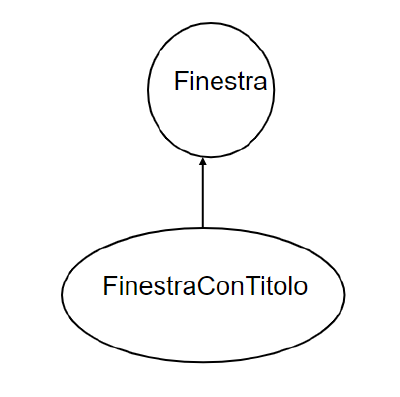
\includegraphics[scale=0.5]{images/ripasso di programmazione II/Finestra.png}
\end{center}
\end{figure}

\nt{In Java l'ereditarietà è singola, per cui ogni classe ha un solo genitore\footnote{E ogni classe discende dalla classe Object}.}

\section{Tipi e metodi}

\dfn{Controllo dei tipi}{Java effettua un controllo statico per i tipi (prima dell'esecuzione). Il \textbf{checking} controlla che per una variabile si  chiami un metodo definito per la classe di quella variabile. }

\dfn{Polimorfismo}{Un oggetto può avere \underline{più} di un tipo. Per esempio un oggetto di tipo E che è figlio di un oggetto di tipo C ha entrambi i tipi (E e C). Dato il tipo di una varabile x (A) e un espressione di tipo (B), x = expr è legale se e solo se A = B oppure se B è una sottoclasse di A.}

\cor{Upcasting e downcasting}{L'\textbf{upcasting} è un movimento da un tipo specifico a uno più generico. Questo assegnamento è sempre legale, per esempio, tutti i cani (specifico) sono animali (generico) oppure tutti i rettangoli (specifico) sono poligoni (generico). Se si effettua un upcasting non si possono più utilizzare i metodi della sottoclasse.

Il \textbf{downcasting} è l'operazione opposta.}

\cor{Overriding}{L'\textbf{overriding} permette a una sottoclasse di sovrascrivere un metodo di una sovraclasse. Per fare ciò si scrive nella sottoclasse un metodo con una firma  uguale a un metodo della sovraclasse e si cambia il corpo. Un classico esempio è la funzione toString.}

\nt{Di default toString restituisce il nome della classe + @ + codici alfanumerici}

\cor{Super}{Si può usare il codice della classe genitore nella classe figlio mediante la classe \textbf{super}. Normalmente se si vuole utilizzare super lo si deve fare come prima cosa. Se non esiste una classe super nel genitore si può causare un loop infinito.}

\dfn{Visibilità}{
\begin{itemize}
    \item \textbf{private}: si vede solo all'interno della classe;
    \item \textbf{protected}: visibile da classi e sottoclassi nello stesso package;
    \item \textbf{public}: visibile da tutti.
\end{itemize}
}

\dfn{Binding dinamico}{Nel \textbf{binding dinamico} si crea un legame durante l'esecuzione. Questo avviene in quasi tutti i linguaggi a oggetti (eccezione C++). In C++ si deve ricorrere all'upcasting. In java non è presente il binding dinamico con le variabili.}

\section{Programmare con l'ereditarietà}

Per ricapitolare, i linguaggi a oggetti:

\begin{itemize}
    \item hanno una struttura modulare;
    \item implementano tipi di dati astratti;
    \item offrono gestione automatica della memoria (garbage collector);
    \item hanno classi;
    \item ereditarietà singola o multipla;
    \item polimorfismo e binding dinamico.
\end{itemize}

\dfn{Riuso del software}{Il programmare a oggetti rende possibile riusare il software:

\begin{itemize}
    \item con il \textbf{contenimento} si definiscono nuove classi i cui oggetti sono già compresi in altre classi. Per esempio l'\textbf{automobile} ha un \textbf{motore}, ha delle \textbf{ruote}, etc.;
    \item con l'\textbf{ereditarietà} si estendono delle classi già esistenti. Per esempio un \textbf{poligono} può essere un \textbf{triangolo}, un \textbf{parallelogramma}, etc. 
\end{itemize}
}

\dfn{Classi astratte}{Alcuni classi possono essere \textbf{astratte} per cui non è necessario implementare il codice di un metodo in cui si specifica solo la firma. Questi metodi estratti servono da interfaccie di metodi usati dalle sottoclassi. Le classi astratte hanno un \textbf{costruttore}, ma non possono essere istanziate.
}

\dfn{Interfacce}{Le \textbf{interfacce} sono strutture simili a delle classi, ma possono contenere solo metodi astratti.}

\nt{Un programma può implementare più di un'interfaccia.}

\subsection{Reflection}

\dfn{Reflection}{La reflection consiste nell'interrogare un oggetto per accertarne alcune caratteristiche.}

\cor{instanceof}{
Per essere sicuri che la classe di un oggetto, a runtime, sia corretta si usa la instanceof. instanceof restituisce true se l'oggetto è istanza di un certa classe, false altrimenti.
}

\nt{instanceof è un particolare tipo di reflection.}

\dfn{La classe Class}{
In java la classe Class contiene tutte le classi C usate in un programma. Rappresenta il \textit{tipo} di un oggetto.
}

\cor{isInstance}{
isInstance è un metodo di Class che funziona come una versione dinamica di instanceof.
}

\cor{getClass}{getClass è un metodo che restutuisce la classe dell'oggetto su cui è invocato.}

\cor{getName}{getName è un metodo che restutuisce, come stringa, il nome dell'oggetto su cui è invocato.}

\cor{forName}{forName è un metodo che carica una classe.}

\cor{getSuperclass}{getSuperclass è un metodo che restutuisce la sopraclasse dell'oggetto su cui è invocato.}

\cor{newInstance}{newInstance è un metodo che crea un nuovo oggetto con la stessa classe dell'oggetto su cui è invocato.}

\nt{newInstance non viene mai usato, perchè si preferisce usare "new"}.

\dfn{java.lang.reflect}{
Il package java.lang.reflect contiene le classi Field, Methods e Constructor.

\paragraph{Class contiene:}
\begin{itemize}
    \item getFields: restituisce un array con i campi della classe su cui è invocato;
    \item getMethods: restituisce un array con i metodi della classe su cui è invocato;
    \item getConstructor: restituisce un array con i costruttori della classe su cui è invocato.
\end{itemize}

\paragraph{Methods contiene:}
\begin{itemize}
    \item getParameterTypes;
    \item invoke.
\end{itemize}

}

\section{Trattamento delle eccezioni}

Durante l'esecuzione di un programma possono verificarsi degli errori.

\begin{itemize}
    \item errori di programmazione;
    \item dati errati in ingresso.
\end{itemize}

\nt{Ci vuole una separazione tra la gestione degli errori e i risultati dei metodi.}

\dfn{Le eccezioni}{Il meccanismo delle eccezioni serve per gestire gli errori veri e propri e anche i casi straordinari.}

\cor{Soluzione banale}{
La prima soluzione che si impara è quella di restituire un valore riservato che indica il successo o il fallimento.
}

\nt{Tuttavia non sempre questo è possibile.}

\dfn{Throw, try e catch}{
Il costrutto throw serve per lanciare le eccezioni. Il costrutto try serve per eseguire istruzioni che potrebbero lanciare eccezioni e catturarle con il costrutto catch (exception handler).
}

\nt{Le eccezioni hanno un determinato tipo (sono oggetti throwable\footnote{Errori irreparabili o eccezioni}). Inoltre gli errori hanno un campo message che specifica il perchè l'errore è avvenuto.}

\dfn{Finally}{Il costrutto finally è sempre eseguito (anche se non sono sollevate eccezioni).}

\ex{Chiusura di un file}{
Le modifiche a un file non sono permanenti finchè non si chiude. In questo caso è utile utilizzare il costrutto finally per chiudere il file sia nel caso in cui non si siano verificate eccezioni sia nel caso ne siano state sollevate.
}

\dfn{Definizione di eccezioni}{Si possono definire eccezioni personalizzate che andranno a estendere Exception o RuntimeException.}

\nt{
\paragraph{Alcuni suggerimenti:}
\begin{itemize}
    \item le eccezioni non devono essere gestite in modo troppo frammentario;
    \item mettere i catch più specifici per primi e i più generici per ultimi;
    \item non si devono silenziare le eccezioni;
    \item se si cattura un errore è preferibile essere severi;
    \item a volte conviene passare un'eccezione invece di gestirla subito.
\end{itemize}
}

\section{Gestione della memoria}

\dfn{Compilazione}{
La compilazione dei programmi scritti in Java prende in input il codice sorgente e restituisce in output il byte code (eseguibile su differenti S.O.).
}

\begin{figure}[ht]
\caption{Come viene compilato un programma Java}
\begin{center}
    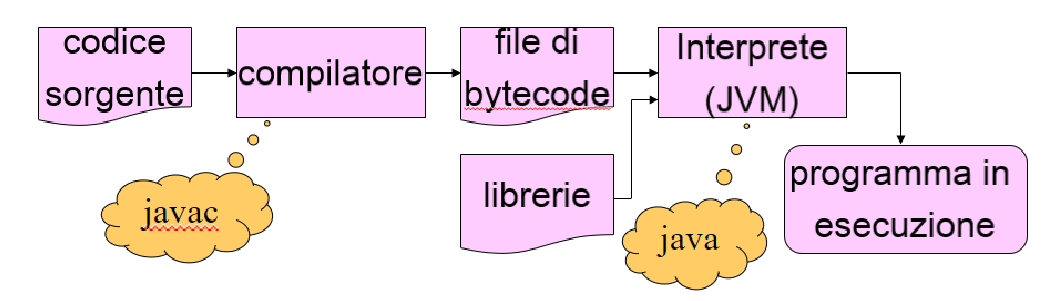
\includegraphics[scale=0.3]{images/ripasso di programmazione II/Compilazione.png}
\end{center}
\end{figure}

\nt{Alcuni IDE, come IntelliJ, automatizzano questo processo.}

\dfn{Memoria della JVM}{
La memoria della JVM è organizzata in:
\begin{itemize}
    \item [$\Rightarrow$] memoria statica: mantiene tutte le parti statiche del programma (alcune variabili, costanti, il codice delle clssi, etc.);
    \item [$\Rightarrow$] stack: è gestito come una pila LIFO (Last In First Out), mantiene i record di attivazioni;
    \item [$\Rightarrow$] heap: presenta il garbage collector e mantiene i dati creati dinamicamente.
\end{itemize}
}

\nt{I metodi che non hanno bisogno di accedere allo stato di un oggetto vanno dichiarati static}

\dfn{Record di attivazione (frame)}{
I record di attivazione contengono i dati necessari a gestire l'esecuzione di un metodo. Contengono:
\begin{itemize}
    \item parametri formali;
    \item varabili locali;
    \item risultato di ritorno (per metodi non-void);
    \item l'indirizzo di ritorno.
\end{itemize}
}

\dfn{Variabili statiche e di istanza}{
\paragraph{Variabili statiche:} c'è una sola copia di queste variabili ed è condivisa fra tutti gli oggetti di una determinata classe.
\paragraph{Variabili di istanza (o dinamiche):} memorizzano lo stato degli oggetti. Ogni oggetto ne ha una copia nel heap.
}
\chapter{Tipi generici e collezioni}

Si vuole poter lavorare in modo "safe" con i tipi di dati senza dover costantemente controllare i tipi di dato.

\section{Tipi generici}

\dfn{Tipi generici}{
I tipi generici si usano per scrivere codice generico applicabile a più tipi di dati (riusabilità del codice). Il tipo E fa un match con qualunque tipo di dato non primitivo al momento della compilazione.

I generici sono stati introdotti per fare inferenza in fase di type checking statico.
}

\nt{Solitamente per i tipi generici si usa la lettera E, ma è solo una convenzione. Qualunque lettera va bene.}

\nt{Si potrebbe usare il tipo Object, ma ciò ha delle limitazioni: per esempio, in un array, possono essere inseriti elementi di tipi diversi. Ovviamente si può usare la reflection, ma ciò è scomodo e inefficiente.}

\ex{ArrayList}{
La classe ArrayList è generica, per cui può contenere oggetti di qualunque tipo. Tuttavia se non si specifica il tipo (ArrayList a = new ArrayList();) verrà considerato Object causando i problemi visti sopra.
}

\dfn{Tipi parametrici}{
Un tipo parametrico è una classe in cui è specificato il tipo generico da inferire.
}

\ex{ArrayList parametrico}{ArrayList$<$Double$>$ a = new ArrayList$<$Double$>$;}

\nt{Si possono creare classi generiche mettendo il parametro E nel nome della classe ($<$E$>$).}

\dfn{Tipo grezzo}{Il compilatore non ragiona in termini di tipi generici. Quindi il compilatore li trasforma in tipi grezzi (raw types), ossia unicamente il tipo della classe senza i parametri.}

\ex{ArrayList}{Quindi: 

ArrayList$<$String$>$ a = new ArrayList$<$String$>$

ArrayList$<$Double$>$ a = new ArrayList$<$Double$>$

hanno lo stesso tipo ArrayList.
}

\nt{Non si possono avere metodi statici con tipi generici all'interno delle classi che usano quei tipi.}

\section{Collezioni}

\dfn{Collezioni}{
Java fornisce un insieme di classi che realizzano strutture dati utili (le collezioni), come 
liste o insiemi.
}

\begin{figure}[h]
    \caption{Le collezioni}
    \begin{center}
        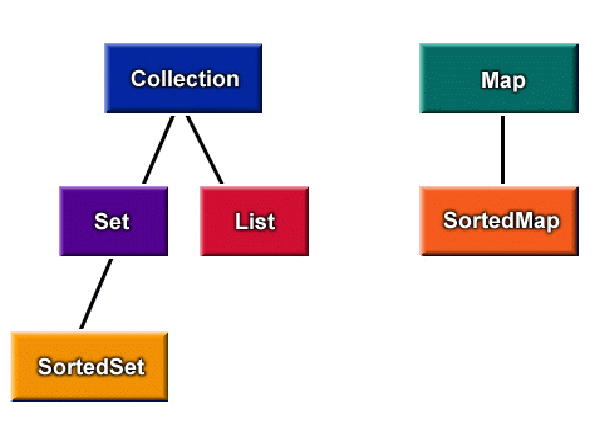
\includegraphics[scale=0.35]{images/Tipi generici e collezioni/Collezioni.png}
    \end{center}
\end{figure}

\nt{Queste sono tutte interfacce:
    \begin{itemize}
    \item \textbf{Collection}: un arbitrario gruppo di oggetti;
    \item \textbf{List}: un gruppo ordinato di oggetti;
    \item \textbf{Set}: un gruppo di oggetti senza duplicati;
    \item \textbf{Map}: una collezione di coppie chiave-valore.
\end{itemize}}

\dfn{Iteratori}{
Un iteratore è un oggetto che permette di scorrere una collezione, ottenendo gli elementi uno alla volta.
Il metodo iterator<> della classe Collection restituisce un iteratore per la collezione.
Si può "ciclare" su una collezione usando un iteratore con next() o con il for each.
}

\nt{Gli array mantengono sempre il loro tipo (a runtime), mentre le collezioni no.}

\dfn{Il tipo jolly (wildcard)}{
Per definire una collection di qualunque generico su usa la notazione collection$<$?$>$.
In una collezione di ? non si può aggiungere nulla, ma si può rimuovere.
}
\chapter{Classi innestate e lambda expression}

\nt{Le lambda expression e, in generale, il $\lambda$-calcolo sono spiegati in dettaglio nei corsi "Linguaggi e paradigmi di programmazione" e "Metodi formali dell'informatica".}

\section{Classi innestate}

Le classi possono essere dichiarate:
\begin{itemize}
    \item all'interno di altre classi in qualità di membri;
    \item all'interno di blocchi di codice.
\end{itemize}

\dfn{Classi innestate}{
    Le classi innestate sono utili per:
    \begin{itemize}
        \item definire tipi strutturati visibili all'interno di gruppi correlati;
        \item connettere in modo semplice oggetti correlati;
        \item information hiding di tipi di dati.
    \end{itemize}
    Il nome di una classe innestata è: NomeContenitore.NomeInnestata. 
}
\nt{La visibilità di una classe innestata è \textit{almeno} la stessa della classe che la contiene.}

\nt{Se non serve dare un nome alle classi innestate
(perché usate in un solo punto del codice della
classe contenitrice) le si può definire come anonime,
per compattezza. Però per questioni di leggibilità si
consiglia di definire classi anonime solo se hanno
poche linee di codice.}

\section{Lambda expression}

\dfn{Lambda expression}{
    Le lambda expression sono utili per implementare interfacce funzionali (cioè interfacce con un solo metodo astratto) in modo compatto:
    \begin{itemize}
        \item possono avere o non avere parametri;
        \item possono avere o non avere un tipo di ritorno.
    \end{itemize}
}
\nt{Se il body ha una sola istruzione e restituisce un valore (non void) si possono omettere le parentesi graffe e la keyword \texttt{return}.}

\section{Input/Output}

\dfn{I/O}{
Le operazioni di I/O avvengono attraverso \textit{stream}:
successioni di byte che rappresentano i dati in input o
in output. Gli stream possono essere combinati. Ci sono due tipi di stream:
\begin{itemize}
    \item \textit{byte stream}: stream di byte;
    \item \textit{character stream}: stream di caratteri.
\end{itemize}
Esistono oltre 60 classi di I/O divise in due gerarchie:    
\begin{itemize}
    \item \texttt{InputStream} e \texttt{OutputStream} per i byte;
    \item \texttt{Reader} e \texttt{Writer} per i caratteri.
\end{itemize}
    }

\nt{
    Sorgente e destinazione di un flusso di byte o di caratteri possono essere:
    \begin{itemize}
        \item \texttt{File}: file sul disco;
        \item \texttt{Array}: array di byte o di caratteri;
        \item \texttt{String}: stringa di caratteri;
        \item \texttt{Pipe}: stream di byte o di caratteri in memoria.
    \end{itemize}
}

\dfn{Input a caratteri}{
    La classe read è la classe astratta che rappresenta un
    generico stream di caratteri. I metodi più importanti
    sono:
    \begin{itemize}
        \item \texttt{int read()}: legge un carattere e lo restituisce come intero;
        \item \texttt{int read(char[] c)}: legge un array di caratteri e restituisce il numero di caratteri letti;
        \item \texttt{int read(char[] c, int off, int len)}: legge un array di caratteri a partire da un offset e restituisce il numero di caratteri letti.
    \end{itemize}
    La classe InputStreamReader è una classe che converte un
    InputStream in un Reader.
}

\dfn{Output a caratteri}{
    La classe \texttt{Writer} è la classe astratta che rappresenta un generico stream di caratteri. I metodi più importanti sono:
    \begin{itemize}
        \item \texttt{void write(int c)}: scrive un carattere;
        \item \texttt{void write(char[] c)}: scrive un array di caratteri;
        \item \texttt{void write(char[] c, int off, int len)}: scrive un array di caratteri a partire da un offset;
        \item \texttt{void flush()}: svuota il buffer di output;
        \item \texttt{void close()}: chiude lo stream.
    \end{itemize}
    La classe OutputStreamWriter è una classe che converte un OutputStream in un Writer.
}

\dfn{Buffer}{
    Un buffer è un'area di memoria temporanea dove vengono
    memorizzati i dati prima di essere letti o scritti. I
    vantaggi dell'utilizzo di un buffer sono:
    \begin{itemize}
        \item riduzione del numero di accessi al disco;
        \item riduzione del tempo di esecuzione.
    \end{itemize}
}

\nt{
    I flussi standard di input e output sono:
    \begin{itemize}
        \item \texttt{System.in}: flusso di input standard;
        \item \texttt{System.out}: flusso di output standard;
        \item \texttt{System.err}: flusso di errori standard.
    \end{itemize}
}

\subsection{Oggetti}

\dfn{I/O di oggetti}{
    Con ObjectInputStream e ObjectOutputStream è possibile
    leggere e scrivere oggetti. Per poter scrivere un oggetto
    su un file è necessario che la classe dell'oggetto sia
    serializzabile, cioè che implementi l'interfaccia
    \texttt{Serializable}. L'interfaccia Serializable è una
    \textit{marker interface}, cioè un'interfaccia senza metodi.

}

\nt{
    Per leggere e scrivere oggetti su un file si usano i metodi:
    \begin{itemize}
        \item \texttt{void writeObject(Object o)}: scrive un oggetto;
        \item \texttt{Object readObject()}: legge un oggetto.
    \end{itemize}
}

\subsection{File}

\dfn{File}{
    Un file è una sequenza di byte memorizzata su un dispositivo
    di memorizzazione permanente. Un file è caratterizzato da:
    \begin{itemize}
        \item nome;
        \item dimensione;
        \item tipo;
        \item posizione.
    \end{itemize}
    I file possono essere:
    \begin{itemize}
        \item \textit{testuali}: contengono caratteri;
        \item \textit{binari}: contengono byte.
    \end{itemize}
}

\nt{
Per leggere e scrivere file si usano le classi:
\begin{itemize}
    \item \texttt{File}: rappresenta un file o una directory;
    \item \texttt{FileReader} e \texttt{FileWriter}: leggono e scrivono file di caratteri;
    \item \texttt{FileInputStream} e \texttt{FileOutputStream}: leggono e scrivono file di byte.
\end{itemize}
}

\dfn{Scanner}{
    La classe \texttt{Scanner} permette di leggere file di caratteri o di byte. I metodi più importanti sono:
    \begin{itemize}
        \item \texttt{String nextLine()}: legge una riga;
        \item \texttt{String next()}: legge una parola;
        \item \texttt{int nextInt()}: legge un intero;
        \item \texttt{double nextDouble()}: legge un double;
        \item \texttt{boolean hasNext()}: verifica se ci sono altri dati da leggere.
    \end{itemize}
}
\chapter{Interfacce grafiche}

\dfn{GUI}{
    Una GUI (Graphical User Interface) è un'interfaccia utente che permette l'interazione uomo-macchina in modo visuale utilizzando rappresentazioni grafiche piuttosto che utilizzando una interfaccia a riga di comando.
}

\nt{Nelle prime versioni di Java (1.0, 1.1) era presente la libreria AWT (Abstract Window Toolkit) che permetteva di creare interfacce grafiche. Questa libreria era basata sulle API native del sistema operativo.}

\begin{figure}[h]
    \centering
    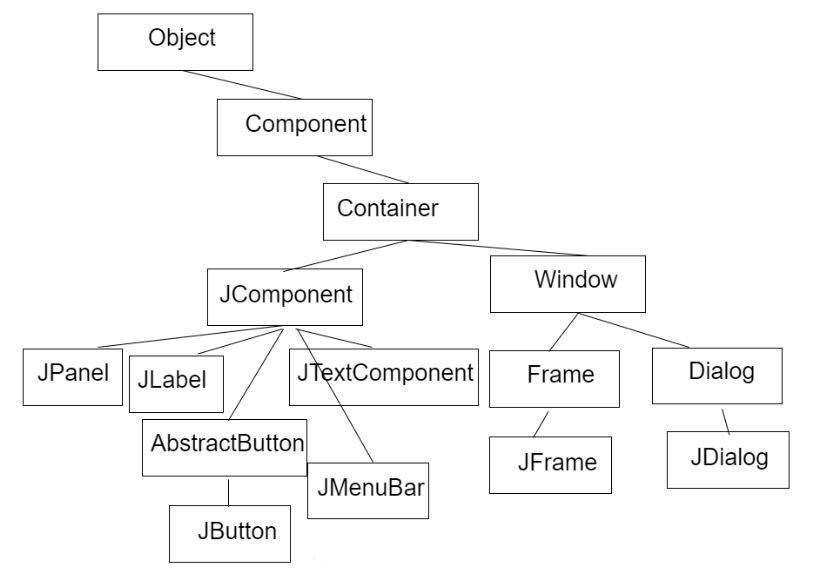
\includegraphics[scale=0.4]{images/Interfacce grafiche/Componenti.png}
    \caption{Gerarchia delle classi di interfaccia grafica}
\end{figure}

\section{SWING}

\dfn{JFrame}{
    Un JFrame è un contenitore che permette di creare una finestra.
    Si possono utilizzare diversi layout.

    La sintassi è:
    \begin{itemize}
        \item \texttt{JFrame frame = new JFrame("Titolo");}
        \item \texttt{frame.setSize(300, 300);}
        \item \texttt{frame.setVisible(true);}
        \item \texttt{JLabel label = new JLabel("Testo");}
        \item \texttt{frame.add(label);}
    \end{itemize}
}

\dfn{Event-driven programming}{
    L'event-driven programming è un paradigma di programmazione in cui il flusso di esecuzione del programma è determinato dagli eventi che avvengono.
    Un evento è un segnale che indica che qualcosa è accaduto.
    Un evento può essere generato da un utente (click del mouse, pressione di un tasto, ...) o da un altro programma.

    \begin{enumerate}
        \item L'applicazione crea gli event-handlers;
        \item L'applicazione registra gli event-handlers\footnote{Questo significa
        che ogni event-handler è legato a un tipo di evento.}.
    \end{enumerate}

}

\begin{figure}[h]
    \centering
    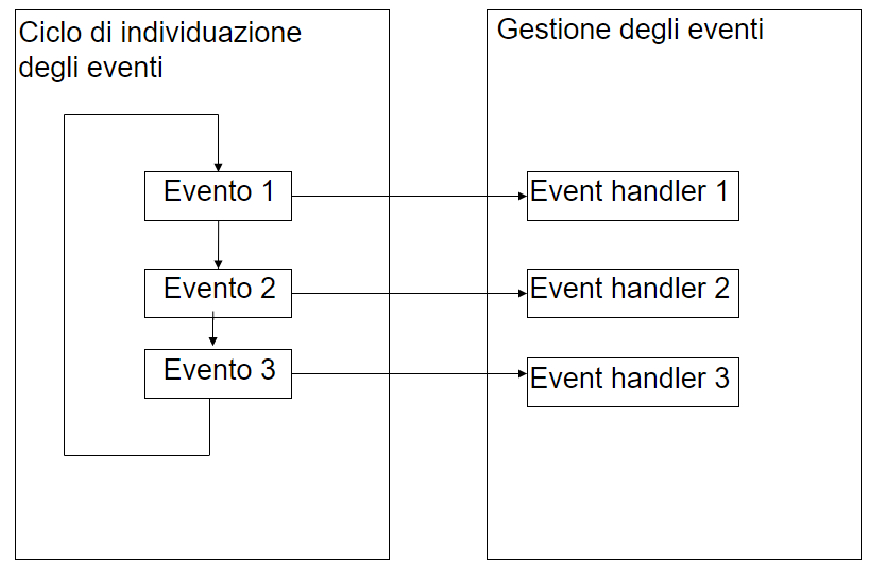
\includegraphics[scale=0.4]{images/Interfacce grafiche/Event driven.png}
    \caption{Eventi}
\end{figure}

\nt{Il ciclo degli eventi è un concetto astratto.}

\dfn{Gestione degli eventi}{
    Gli eventi sono passati da un oggetto a un listener che lo gestisce.
    Il listener deve essere registrato presso la sorgente dell'evento.
    Il passaggio dell'evento causa l'invocazione di un metodo del listener.
}

\cor{Listener}{
    Esistono differenti \texttt{interface}:
    \begin{itemize}
        \item ActionListener: gestisce gli eventi generati da un componente che genera azioni (es. JButton);
        \item MouseListener: gestisce gli eventi generati da un componente che genera azioni del mouse;
        \item MouseMotionListener: gestisce gli eventi generati da un componente che genera azioni del mouse;
        \item WindowListener: gestisce gli eventi generati da un componente che genera azioni della finestra (JFrame).
    \end{itemize}
}

\dfn{Adapters}{
    Gli adapters sono classi che implementano un'interfaccia e forniscono un'implementazione vuota di tutti i metodi.
    Questo permette di implementare solo i metodi che interessano.
}

\nt{Ci possono essere casi con ogni bottone associato al proprio listener. Oppure più bottoni con lo stesso listener.}


\section{Pattern Observe - Observable}

\dfn{Pattern Observe - Observable}{
    Il pattern Observe - Observable è un pattern che serve per rendere più modulare 
    il codice e per permettere la comunicazione tra oggetti. Viene usato anche in altri ambiti,
    ma in questo corso ci occuperemo del suo uso in relazione alla GUI.
}

\nt{In Java esistono gli oggetti \texttt{Observer} e \texttt{Observable} che implementano questo pattern,
tuttavia sono deprecate.
}

\dfn{Observer}{
    L'Observer osserva uno o più oggetti Observable, registrandosi presso di essi.
}

\dfn{Observable}{
    L'Observable è un oggetto che può essere osservato da uno o più Observer.
    Quando l'Observable cambia stato, notifica gli Observer.
}

\nt{La notifica viene effettuata tramite il metodo \texttt{update()}.}

\cor{Metodi di Observer}{
    \begin{itemize}
        \item \texttt{update(Observable o, Object arg)}: viene invocato quando l'Observable cambia stato.
    \end{itemize}
}

\cor{Metodi di Observable}{
    \begin{itemize}
        \item \texttt{addObserver(Observer o)}: aggiunge un Observer;
        \item \texttt{deleteObserver(Observer o)}: rimuove un Observer;
        \item \texttt{notifyObservers()}: notifica tutti gli Observer;
        \item \texttt{notifyObservers(Object arg)}: notifica tutti gli Observer con un argomento;
        \item \texttt{deleteObservers()}: rimuove tutti gli Observer.
    \end{itemize}
}

\begin{figure}[h]
    \centering
    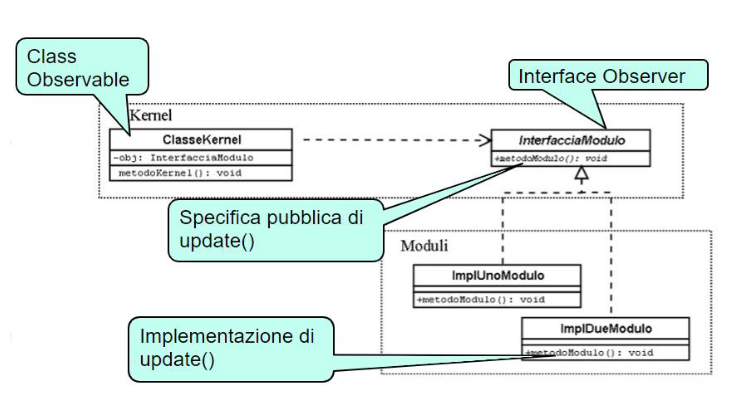
\includegraphics[scale=0.4]{images/Interfacce grafiche/Observer - Observable.png}
    \caption{Pattern Observer - Observable}
\end{figure}

\nt{Le moderne librerie grafiche JavaFX utilizzano questo pattern internamente.}

\section{Pattern MVC}

\dfn{MVC}{
    Un programma si compone di:
    \begin{itemize}
        \item Model: rappresenta i dati e le operazioni che possono essere effettuate su di essi;
        \item View: visualizza i dati e permette l'interazione con l'utente;
        \item Controller: gestisce gli eventi generati dall'utente e aggiorna il model e la view.
    \end{itemize}
}

\nt{Il model è collegato alla view tramite il controller.}

\begin{figure}
    \begin{center}
        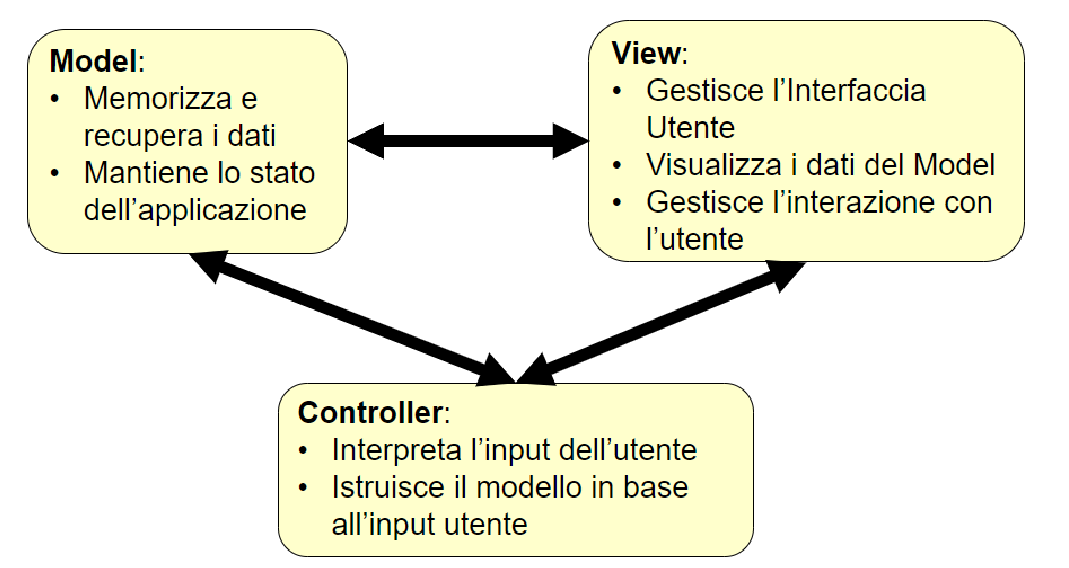
\includegraphics[scale=0.25]{images/Interfacce grafiche/MVC.png}
    \end{center}
    \caption{Pattern MVC}
\end{figure}

\section{JavaFX}

\dfn{JavaFX}{
    JavaFX è una libreria grafica per lo sviluppo di GUI:
    \begin{itemize}
        \item[$\Rightarrow$] per usarla bisogna aver compreso SWING;
        \item[$\Rightarrow$] separa il contenuto dalla sua visualizzazione tramite fogli
        di stile CSS;
        \item[$\Rightarrow$] permette il binding di properties dei Model;
        \item[$\Rightarrow$] offre classi/interfacce che implementano Observer/Observable;
        \item[$\Rightarrow$] permette di creare interfacce grafiche tramite XML. 
    \end{itemize}
}

\cor{Componenti di JavaFX}{
    \begin{itemize}
        \item \texttt{Stage}: rappresenta una finestra (simile a JFrame);
        \item \texttt{Scene}: rappresenta il contenuto di una finestra.
    \end{itemize}

    La struttura della GUI è gerarchica: nel pannello della scene si inseriscono i
    componenti figli. In uno stage ci può essere una sola scene.
}

\dfn{Form (moduli)}{
    In JavaFX si possono anche creare dei form basati su:
    \begin{itemize}
        \item \texttt{GridPane}: per inserire i componenti grafici in una griglia;
        \item \texttt{Label}: titoli dei campi;
        \item \texttt{TextField}: campi di input;
        \item \texttt{Button}: pulsanti;
        \item \texttt{Text}: testo non modificabile (output). 
    \end{itemize}
}

\dfn{Uso di CSS}{
    Per utilizzare CSS in JavaFX bisogna:
    \begin{itemize}
        \item Creare un file CSS;
        \item Creare un oggetto \texttt{Scene} e associargli il file CSS;
        \item Associare la scena allo stage.
    \end{itemize}
}

\section{JavaFXML}

\dfn{JavaFXML}{
    JavaFXML è un linguaggio di markup basato su XML che permette di creare interfacce grafiche.
    Permette di separare la struttura della GUI dal codice Java.
    Permette di creare interfacce grafiche in modo dichiarativo.
    Permette di utilizzare CSS.
    Permette di utilizzare il pattern MVC.
}

\subsection{Scene Builder}

\dfn{Scene Builder}{
    Scene Builder è un tool che permette di creare interfacce grafiche in modo visuale.
    Permette di creare interfacce grafiche in modo dichiarativo.
}

\subsection{Properties}

\dfn{Java beans}{
    Un Java bean è una classe che:
    \begin{itemize}
        \item Ha un costruttore senza argomenti;
        \item Ha metodi getter e setter per ogni attributo;
        \item Implementa Serializable.
    \end{itemize}
}

\dfn{Properties}{
    Una property è un attributo di un Java bean.
    Le properties di libreria servono per:
    \begin{itemize}
        \item Binding: permette di collegare due properties;
        \item Listener: permette di associare un listener ad una property.
    \end{itemize}
    
}

\ex{ObservableValue<T>}{
    L'interfaccia \texttt{ObservableValue<T>} è un'interfaccia generica
    che rappresenta una property. Ha i seguenti metodi:
    \begin{itemize}
        \item \texttt{getValue()}: ritorna il valore della property;
        \item \texttt{addListener(ChangeListener<? super T> listener)}: aggiunge un listener;
        \item \texttt{removeListener(ChangeListener<? super T> listener)}: rimuove un listener;
        \item \texttt{addListener(InvalidationListener listener)}: aggiunge un listener;
        \item \texttt{removeListener(InvalidationListener listener)}: rimuove un listener.
    \end{itemize}
}

\ex{ChangeListener}{
    L'interfaccia \texttt{ChangeListener<T>} è un'interfaccia generica
    che rappresenta un listener per una property. Ha il seguente metodo:
    \begin{itemize}
        \item \texttt{changed(ObservableValue<? extends T> observable, T oldValue, T newValue)}: viene invocato quando il valore della property cambia.
    \end{itemize}
}

\dfn{Properties in JavaFX}{
    In JavaFX esistono le seguenti properties:
    \begin{itemize}
        \item \texttt{SimpleStringProperty}: rappresenta una property di tipo String;
        \item \texttt{SimpleIntegerProperty}: rappresenta una property di tipo Integer;
        \item \texttt{SimpleDoubleProperty}: rappresenta una property di tipo Double;
        \item \texttt{SimpleBooleanProperty}: rappresenta una property di tipo Boolean.
    \end{itemize}
}
\afterpage{\blankpage}
\chapter{Laboratorio}

\section{Lezione 1}

\subsection{La piattaforma IntelliJ}

\dfn{IDE}{
Quando si sviluppa un software (SW) di grandi dimensioni è necessario utilizzare un \textbf{IDE}\footnote{Integrated development environment}. 
}

\nt{L'IDE offre supporto alla compilazione e all'esecuzione dei programmi, a caricarli sul web, etc.}

\dfn{IntelliJ}{\textbf{IntelliJ} offre un editor per lo sviluppo di applicazioni web e standalone.

Le versioni principali sono due:

\begin{itemize}
    \item Community: non permette lo sviluppo web;
    \item ULTIMATE: è la versione completa ed è gratuita per studenti universitari.
\end{itemize}
}
\cor{}{
IntelliJ organizza tutte le applicazioni in progetti (\textbf{Project}), ognuno dei quali include:
\begin{itemize}
    \item \textit{Source Package (src)}: il codice sorgente, ossia le classi java;
    \item \textit{External library}: le librerie utilizzate;
    \item altre cartelle.
\end{itemize}
}

\subsection{Installare IntelliJ}

\begin{enumerate}
    \item Come prerequisito bisogna aver installato almeno la \underline{versione 13} di \href{https://www.oracle.com/it/java/technologies/downloads/\#jdk21-windows}{JDK} (meglio se 20 o successiva);
    \item Installare \textbf{JetBrains} Toolbox da questo link: \href{https://www.jetbrains.com/toolbox-app/}{https://www.jetbrains.com/toolbox-app/};
    \item Avviare JetBrains Toolbox;
    \item Cercare e installare \textbf{IntelliJ IDEA ultimate};
    \item Avviare IntelliJ IDEA ultimate;
    \item Cliccare sui tre puntini in basso a sinistra e selezionare Manage Licenses;
    \item Acquisire la licenza di IntelliJ IDEA\footnote{Nota: la licenza è fornita gratuitamente agli studenti universitari, ma deve essere rinnovata ogni anno}.
\end{enumerate}

\nt{Per verificare la propria JDK basta eseguire il comando "java --version" da terminale.}

\subsection{Estensioni utili}

Breve elenco di plugins che possono migliorare la \textbf{quality of life} (QOL).

\begin{itemize}
    \item Atom Material Icons: un set di icone che rende più "vivace" l'ambiente di sviluppo favorendo visivamente il riconoscimento di file e cartelle;
    \item CodeGlance Pro: mostra una "\textbf{mappa}" del proprio codice a destra dello schermo, permettendo una rapida visione d'insieme e la possibilità di spostarsi precisamente usando l'interfaccia grafica;
    \item Conventional Commit: fornisce un completamento per commit "standard" su git;
    \item Key Promoter X: serve per imparare le combinazioni di tasti (\textbf{shortcuts}). Ogni volta che si utilizza il menu testuale viene mostrata l'alternativa con la tastiera insieme a un contatore che segna quanti "miss" di quella shortcut sono stati fatti;
    \item PDF Viewer: permette di visualizzare i file PDF all'interno dell'IDE;
    \item Rainbow CSV: migliora la lettura dei file CSV colorando i vari campi;
    \item Rainbow Brackets: migliora la leggibilità del codice colorando le parentesi.
\end{itemize}

\ex{Per iniziare}{

Per creare un progetto bisogna aprire il menu File $\rightarrow$ New $\rightarrow$ Project. Nel menu che compare si seleziona New Project, con language Java, si definisce il nome del progetto e si clicca su create.

Il progetto nasce con la cartella \textbf{src}. Si possono creare classi, package, etc. facendo clic con il tasto destro all'interno della cartella che si vuole usare.

IntelliJ possiede anche utili funzioni che segnalano gli errori e aiutano con la compilazione. Riguardo all'autocompilazione: può essere usata per creare costruttori, getter, setter, toString, etc.

Quando si compila il programma viene creata la cartella \textbf{out} che contiene i file \textit{.class} del progetto. Essa viene distrutta e ricreata ogni volta che si compila il progetto in modo da eliminare eventuali problemi di dipendenze.
}
\nt{IntelliJ crea e gestisce i progetti in una cartella di default "IdeaProjects".}

\nt{Per convenzione, in un progetto Java, le classi che rappresentano oggetti delle applicazioni vanno inseriti in una cartella \textbf{model}, le classi che gestiscono le operazioni di input/output vanno inseriti in una cartella \textbf{io}.}

\section{Lezione 2}

\section{Lezione 3}

\section{Lezione 4}

\end{document}